\section{Prueba de la interfaz}
\label{sec:UIResults}

En esta sección se va a analizar el funcionamiento general de la interfaz mediante una serie de pruebas centradas en sus funciones principales.

\subsection{Importación de archivos}
\label{sec:PruebasImportacionArchivos}

Cuando el usuario pulsa cualquiera de los botones para importar archivos a su correspondiente base de datos, ya sea la base de datos de los archivos de entrada de datos de la oferta, la de los archivos de entrada de datos de la configuración de la demanda o la de los archivos de resultados, el programa pide al usuario que seleccione el archivo que desea introducir en la base de datos.

Después de seleccionar el archivo, se pregunta al usuario si quiere añadir alguna observación a la entrada que se va a crear en la tabla \texttt{TESTS} de la base de datos correspondiente (Figura~\ref{fig:askForObservations}). 

\begin{figure}[H]
    \centering
    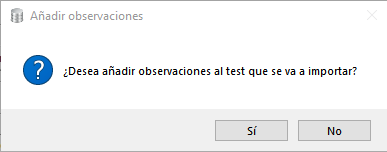
\includegraphics[width=0.6\linewidth]{fig/Interfaz de la aplicación/añadir observaciones.png}
    \caption{Ventana de confirmación para añadir observaciones a la entrada del archivo.}
    \label{fig:askForObservations}
\end{figure}

En caso de que la respuesta por parte del usuario sea positiva, se muestra otra ventana (Figura~\ref{fig:observationsWindow}) en la que el usuario puede escribir la observación que quiere que se almacene en la columna \texttt{OBSERVATIONS} en la tabla \texttt{TESTS} de la base de datos. Después de introducir las observaciones, el programa intenta introducir los datos del archivo seleccionado en la base de datos. 

\begin{figure}[H]
    \centering
    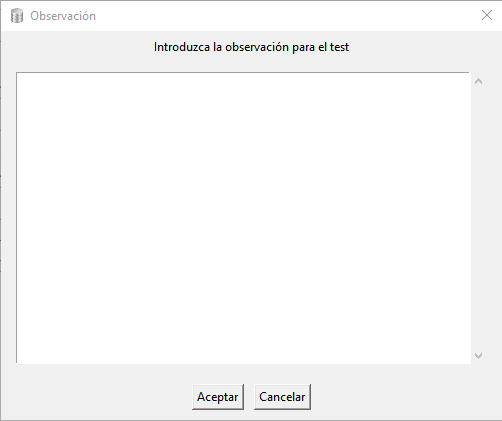
\includegraphics[width=0.6\linewidth]{fig/Interfaz de la aplicación/ventana para añadir observaciones.png}
    \caption{Ventana para añadir observaciones.}
    \label{fig:observationsWindow}
\end{figure}

En caso de que la respuesta por parte del usuario sea negativa, se procede a introducir los datos del archivo seleccionado en la base de datos sin añadir ninguna observación.

Si el programa no ha encontrado problemas al introducirlo, notificará al usuario mediante una ventana de información (Figura~\ref{fig:importSuccess}) que la importación ha sido exitosa. Si por el contrario, la importación ha fallado, también se le notificará al usuario mediante una ventana de error (Figura~\ref{fig:importFailed}). Por último, si el archivo que se intenta introducir en la base de datos ya se encuentra dentro de la base de datos, el programa mostrará que ha habido un error al importar el archivo, haciendo hincapié en que puede que el archivo ya se encuentre en la base de datos (Figura~\ref{fig:importFailedDueDuplicatedFile}). Con estas comprobaciones se ha verificado la detección de los potenciales errores en este proceso.

\begin{figure}[H]
    \centering
    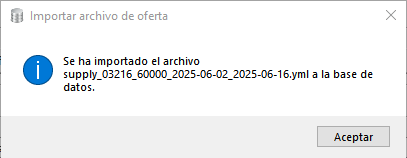
\includegraphics[width=0.5\linewidth]{fig/Interfaz de la aplicación/mensaje de importacion exitosa.png}
    \caption{Ventana de notificación para importación exitosa.}
    \label{fig:importSuccess}
\end{figure}

\begin{figure}[H]
    \centering
    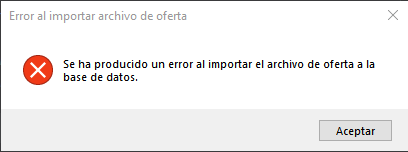
\includegraphics[width=0.5\linewidth]{fig/Interfaz de la aplicación/mensaje de importacion fallida.png}
    \caption{Ventana de notificación para importación fallida.}
    \label{fig:importFailed}
\end{figure}

\begin{figure}[H]
    \centering
    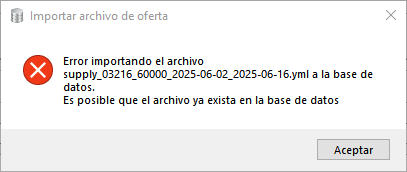
\includegraphics[width=0.5\linewidth]{fig/Interfaz de la aplicación/mensaje de importacion duplicada.png}
    \caption{Ventana de notificación para archivo duplicado.}
    \label{fig:importFailedDueDuplicatedFile}
\end{figure}

\subsection{Exportación de archivos}
\label{PruebasExportacionArchivos}

En caso de que el usuario quiera exportar uno de los archivos almacenados en la base de datos ha de presionar uno de los botones destinados a la exportación de los archivos. Después de presionar uno de los botones, el programa muestra una ventana (Figura~\ref{fig:fileSelectorWindow}) con una lista con los archivos que se encuentran almacenados en la base de datos para que el usuario seleccione cual de ellos es el que quiere exportar. Acto seguido, se le pide al usuario seleccionar la carpeta en la que se va a guardar el archivo exportado. Si la base de datos no contiene ningún archivo almacenado, el programa muestra un mensaje de error indicando que la base de datos se encuentra vacía.

%De igual forma, si el usuario presiona cualquiera de los botones para exportar archivos de la base de datos a un archivo, ya sea un archivo \acrshort{Yaml} en caso de los archivos de entrada de datos de la oferta y la demanda o un \acrshort{CSV} en caso de que el archivo sea un archivo de resultados del simulador, el programa mostrará una ventana (Figura~\ref{fig:fileSelectorWindow}) en la que aparecen los nombres de todos los archivos que haya almacenados en la base de datos para que el usuario seleccione cuál quiere exportar. Después, se le pide al usuario que seleccione la carpeta en la que desea guardar el archivo que se generará. Si la base de datos de la que se quiere extraer un archivo no contiene ninguno, el programa lanzará un mensaje de error indicando al usuario que la base de datos se encuentra vacía.

\begin{figure}[H]
    \centering
    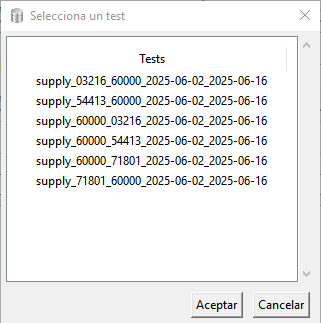
\includegraphics[width=0.5\linewidth]{fig/Interfaz de la aplicación/seleccion de test a exportar.png}
    \caption{Ventana de selección de archivo.}
    \label{fig:fileSelectorWindow}
\end{figure}

Una vez seleccionado el archivo a exportar y la ubicación en la que se va a guardar, el programa comienza a recabar la información almacenada en la base de datos, apoyándose en las tablas auxiliares para saber qué información de la que contienen las tablas de datos pertenece al archivo en cuestión. Una vez recabada la información del archivo, se le da el mismo formato que poseen los datos al procesar un archivo \acrshort{Yaml}. Tras esto, el programa crea el archivo en la ubicación especificada anteriormente e inserta la información a la que previamente se le ha dado el mismo formato que a un archivo \acrshort{Yaml}.

\subsection{Eliminación de archivos de la base de datos}
\label{PruebasEliminacionArchivos}

En caso de que el usuario quiera eliminar un archivo de la base de datos, se debe pulsar uno de los botones dentro de la sección "Eliminar de la base de datos". Tras presionar uno de los botones, aparece una ventana (Figura~\ref{fig:fileSelectorWindow}) para seleccionar qué archivo se desea eliminar. Una vez seleccionado, el programa lanza una serie de sentencias \acrshort{SQL} que se encargan de eliminar el archivo y todos los datos pertenecientes a este, que no estén presentes en ningún otro archivo. Por ejemplo, si en el archivo que se va a eliminar aparece la estación de Atocha y esta se encuentra en otro archivo de los almacenados en la base de datos, no será eliminada. Por el contrario, si, por ejemplo, la estación de Chamartín solo aparece en el archivo que se va a eliminar, esta sí que será eliminada de la tabla \texttt{STATIONS}.

\subsection{Ejecución de sentencias \acrshort{SQL}}
\label{PruebasEjecucionSQL}

El programa también permite la interacción con las bases de datos, mediante sentencias \acrshort{SQL}. Hay 3 formas diferentes de ejecutar estas sentencias: desde las sentencias almacenadas en la memoria del programa, escribiendo la sentencia directamente en el cuadro de texto dentro de la sección "SQL" y ejecutándola en la base de datos a la que vaya dirigida la sentencia, o cargando la sentencia directamente desde un archivo y ejecutándola en la base de datos objetivo. Para la selección de la base de datos se genera una ventana (Figura~\ref{fig:dataBaseSelector}) para seleccionar cuál de las tres es el objetivo de la sentencia \acrshort{SQL}.

\begin{figure}[H]
    \centering
    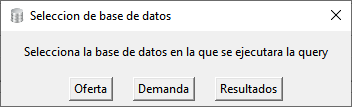
\includegraphics[width=0.5\linewidth]{fig/Interfaz de la aplicación/ventana de seleccion de Db.png}
    \caption{Ventana de selección de la base de datos objetivo.}
    \label{fig:dataBaseSelector}
\end{figure}

Por defecto, en la aplicación hay tres sentencias guardadas en memoria (Figura~\ref{fig:listOfQuerysOnMemory}). Las tres sentencias son para mostrar los archivos almacenados en cada una de las bases de datos. Para usarlas, hay que seleccionar la que se quiera ejecutar del menú desplegable y pulsar el botón ejecutar, que aparece a su derecha. 

\begin{figure}[H]
    \centering
    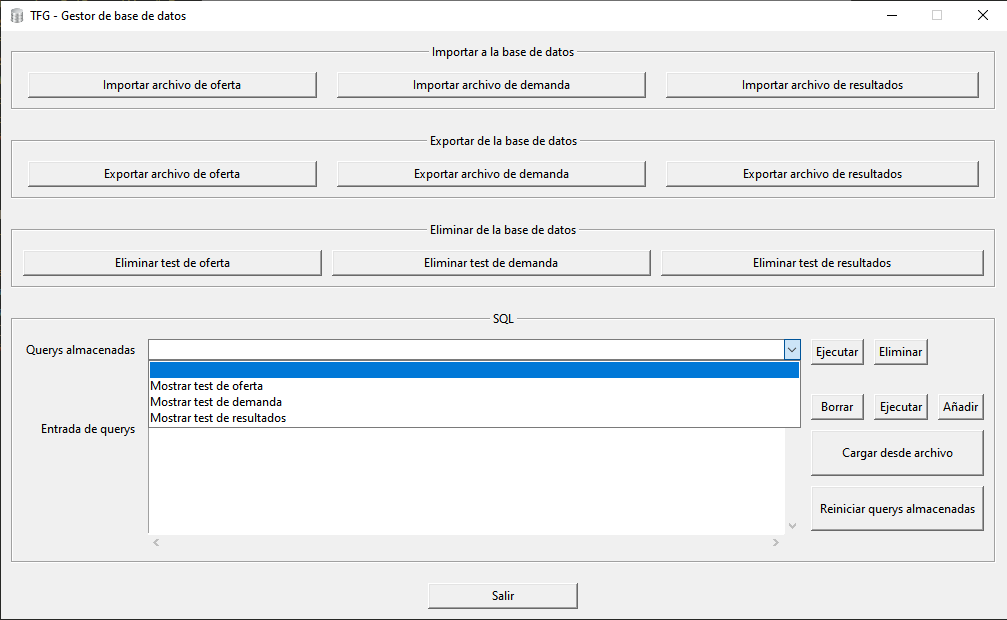
\includegraphics[width=1\linewidth]{fig/Interfaz de la aplicación/lista de consultas guardadas.png}
    \caption{Desplegable con las sentencias almacenadas en la aplicación.}
    \label{fig:listOfQuerysOnMemory}
\end{figure}

Para este ejemplo, se usa la sentencia almacenada "Mostrar test de oferta", cuya sentencia \acrshort{SQL} es la que aparece reflejada en el siguiente listado:

\begin{lstlisting}[language=SQL,
                   frame=none,
                   numbers=none,
                   basicstyle=\ttfamily\normalsize,
                   caption={sentencia "Mostrar test de oferta"},
                   label=src:queryMostrarTestDeOferta,
                   inputencoding=utf8]                   
SELECT *
FROM TESTS
\end{lstlisting}


 Debido a que las sentencias que se incluyen por defecto se encargan de seleccionar datos en la base de datos mediante el comando \acrshort{SQL} \texttt{SELECT}, los datos que devuelva la base de datos se muestran en una ventana aparte, en la que se puede exportar la tabla generada a un archivo \acrshort{CSV}, con un nombre personalizado definido por el usuario. En este caso, en la Figura~\ref{fig:resultsOfQueryOnMemory} se puede observar el resultado de la ejecución de la sentencia "Mostrar test de oferta".

 \begin{figure}[H]
    \centering
    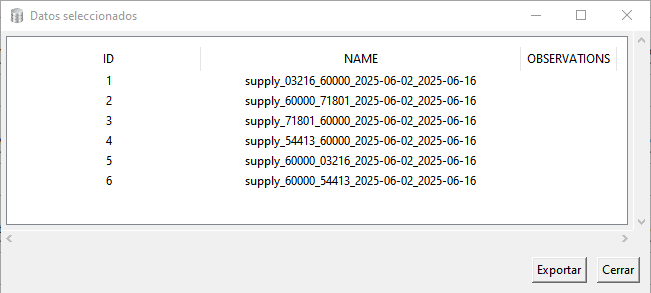
\includegraphics[width=1\linewidth]{fig/Interfaz de la aplicación/resultado de la consulta mostrar tests oferta.png}
    \caption{Ventana con los resultados de la sentencia "Mostrar test de oferta".}
    \label{fig:resultsOfQueryOnMemory}
\end{figure}

Como ya se ha mencionado anteriormente, el usuario de la aplicación también puede escribir sentencias directamente en la interfaz mediante la entrada de texto. El funcionamiento es el siguiente: el usuario introduce la sentencia en el cuadro de texto, y después pulsa el botón "Ejecutar". Acto seguido aparece la ventana para seleccionar la base de datos en la que ejecutar la sentencia (Figura~\ref{fig:dataBaseSelector}). En este caso, como ejemplo, se va a ejecutar la siguiente sentencia \acrshort{SQL}:

\begin{lstlisting}[language=SQL,
                   frame=none,
                   numbers=none,
                   basicstyle=\ttfamily\normalsize,
                   caption={Selección de tests con id < 5},
                   label=src:queryTestId<5,
                   inputencoding=utf8]                   
SELECT * FROM TESTS WHERE ID < 5
\end{lstlisting}

Esta sentencia selecciona los archivos cuyo campo \texttt{ID} tenga un valor inferior a 5. El resultado de la sentencia aparece en la Figura~\ref{fig:queryTestid<5}

\begin{figure}[H]
    \centering
    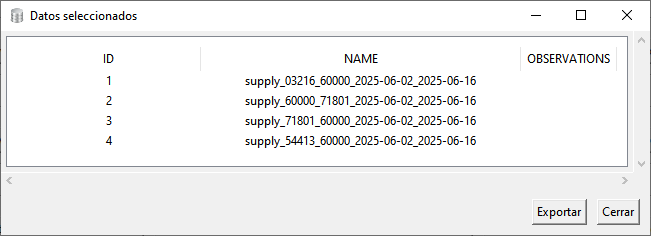
\includegraphics[width=1\linewidth]{fig/Interfaz de la aplicación/resultados de la consulta escrita en la interfaz.png}
    \caption{Ventana con los resultados de la sentencia del Listado~\ref{src:queryTestId<5}.}
    \label{fig:queryTestid<5}
\end{figure}

Además, se pueden importar sentencias desde archivos con extensión \texttt{.sql}. Al importar estos archivos, la sentencia que contengan se muestra en el cuadro de texto. Para ejecutar la sentencia se sigue el mismo procedimiento que en el caso de redactar la sentencia dentro de la interfaz. Como ejemplo, se van a seleccionar las estaciones pertenecientes al ramal con el identificador de valor 10, perteneciente al corredor español, requiriendo a la base de datos el valor de las columnas \texttt{ID}, \texttt{NAME} y \texttt{CITY} de la tabla \texttt{STATIONS} (Figura~\ref{fig:dbSupplySTATIONS}).

Para ello, se emplea la sentencia \acrshort{SQL} del Listado~\ref{src:queryStationsOnPathId10}.

\lstinputlisting[language=SQL, frame=none, numbers=none, basicstyle=\ttfamily\normalsize, caption={Estaciones del ramal con identificador 10}, 
                 label=src:queryStationsOnPathId10, inputencoding=utf8]{auxFiles/Querys de ejemplos/Estaciones ramal id 10.sql}

Al ejecutar la sentencia del Listado~\ref{src:queryStationsOnPathId10}, la aplicación muestra la ventana de la Figura~\ref{fig:resultsOfQueryStationsOnPathId10}, con los datos solicitados a la base de datos de los archivos de entrada de datos de la oferta, en este caso.

\begin{figure}[H]
    \centering
    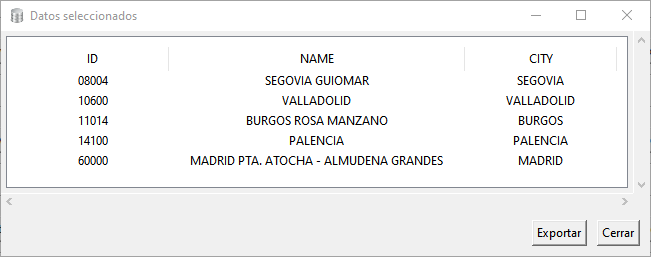
\includegraphics[width=1\linewidth]{fig/Interfaz de la aplicación/Estaciones seleccionadas del ramal con id 10.png}
    \caption{Estaciones pertenecientes al ramal con identificador 10.}
    \label{fig:resultsOfQueryStationsOnPathId10}
\end{figure}

En la Figura~\ref{fig:corridorPaths} se pueden ver todos los ramales del corredor español. El ramal que se encuentra seleccionado corresponde con el ramal que posee el identificador con valor 10. Se puede apreciar que las estaciones que tienen el identificador contenido en el ramal aparecen en la Figura~\ref{fig:resultsOfQueryStationsOnPathId10}, aunque con un orden distinto. Esto se debe a que en el ramal, las estaciones se ordenan según el recorrido; se inicia por la estación de inicio y las siguientes se listan según el trayecto. En cambio, los datos que muestra la ventana de la aplicación se ordenan siempre de manera ascendente según el identificador.

\begin{figure}[H]
    \centering
    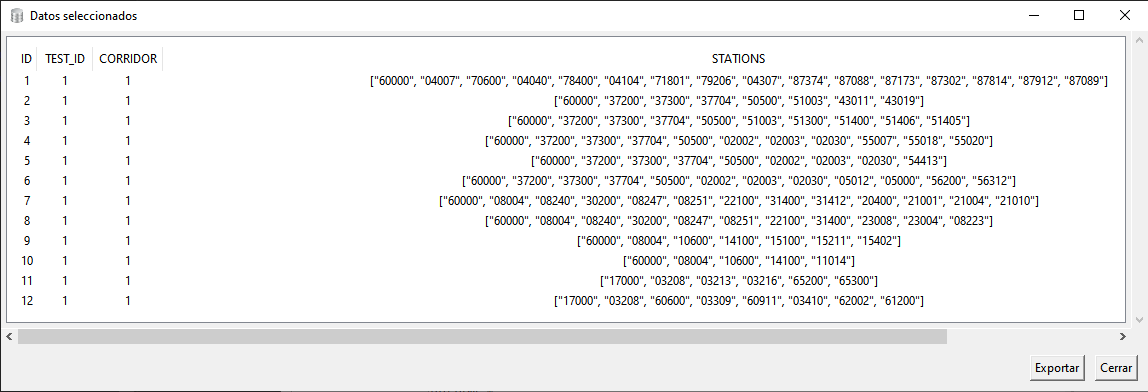
\includegraphics[width=1\linewidth]{fig/Interfaz de la aplicación/ramales del corredor.png}
    \caption{Ramales del corredor español.}
    \label{fig:corridorPaths}
\end{figure}

\subsection{Gestión de sentencias \acrshort{SQL}}
\label{PreubasGestionSQL}

Las sentencias \acrshort{SQL} introducidas en la entrada de texto pueden ser almacenadas en la aplicación para su posterior uso, sin la necesidad de volver a introducirlas. Para ello, una vez escrita la sentencia, pulsamos el botón "Añadir" y, acto seguido, se pide al usuario que seleccione a qué base de datos quiere afectar con esa sentencia cuando sea lanzada desde la memoria y, por último, se pide al usuario que le añada un nombre a esa sentencia. Una vez hecho esto, la sentencia recién guardada aparece en el desplegable de las sentencias almacenadas. Como ejemplo, se ha añadido la sentencia del Listado~\ref{src:queryTestId<5} a la memoria de la aplicación. Al pulsar el botón de añadir, se muestra una ventana para poner el nombre a la sentencia a guardar; en este caso, se le ha puesto el nombre "Seleccionar test con id < 5". Tras nombrar la sentencia, se selecciona a qué base de datos afecta la sentencia y, una vez hecho esto, la sentencia aparece en el menú desplegable junto a las otras sentencias almacenadas en memoria, como se puede ver en la Figura~\ref{fig:queryTestId<5Saved}.

\begin{figure}[H]
    \centering
    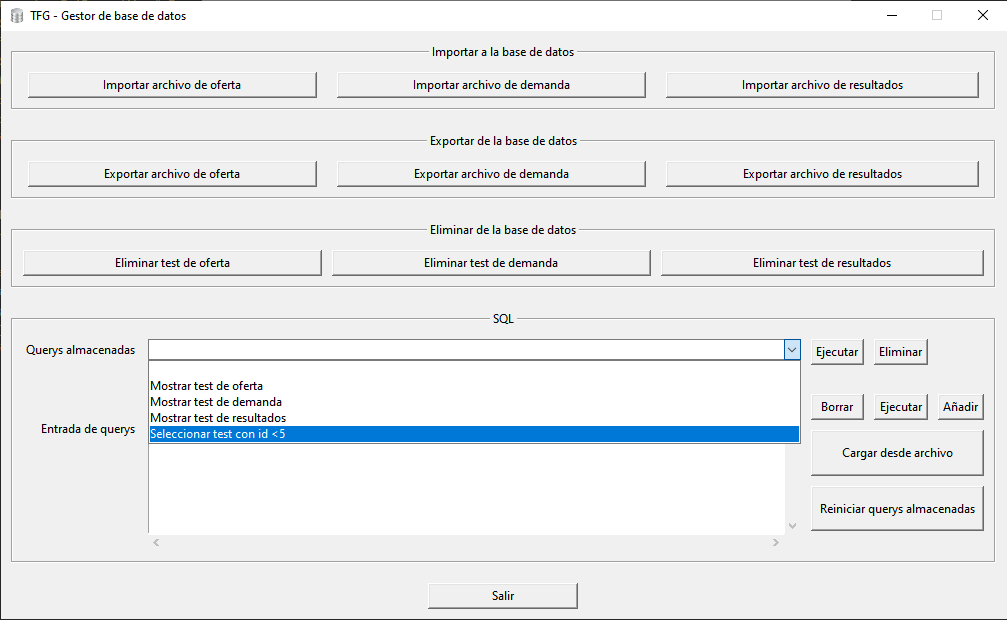
\includegraphics[width=1\linewidth]{fig/Interfaz de la aplicación/nueva lista de consultas guardadas.png}
    \caption{Nueva lista de sentencias guardadas.}
    \label{fig:queryTestId<5Saved}
\end{figure}

\subsection{Generación de \acrshort{CSV} a partir de los datos devueltos por sentencias \acrshort{SQL}}
%\textbf{TEMA: REESCRIBE, FRASE MUY COMPLICADA}
%Empleando la salida de la sentencia \acrshort{SQL} que selecciona las estaciones del ramal con el identificador de valor 10, que se muestran en la Figura~\ref{fig:resultsOfQueryStationsOnPathId10}, se va a generar un archivo \acrshort{CSV} con la funcionalidad de exportar los resultados de las sentencias \acrshort{SQL} que devuelvan datos. En la Tabla~\ref{tab:csvExported} se pueden observar los datos que contiene el archivo \acrshort{CSV}. El archivo se encuentra en el siguiente \href{https://github.com/Sergioba99/TFG-Gestor_De_Bases_de_Datos/blob/master/Archivos%20Yaml%20y%20CSV/Exportados/Vistas%20exportadas/Estaciones%20del%20ramal%20con%20id%2010.csv}{enlace}\footnote{\textbf{Archivo exportado: }\url{https://github.com/Sergioba99/TFG-Gestor\_De\_Bases\_de\_Datos/blob/master/Archivos\%20Yaml\%20y\%20CSV/Exportados/Vistas\%20exportadas/Estaciones\%20del\%20ramal\%20con\%20id\%2010.csv}} del repositorio de GitHub.

Empleando la salida de la sentencia \acrshort{SQL} del Listado~\ref{src:queryStationsOnPathId10}, se va a generar un archivo \acrshort{CSV} con el que verificar el correcto comportamiento de la funcionalidad para exportar los datos devueltos por la ejecución de una sentencia \acrshort{SQL} (Figura~\ref{fig:resultsOfQueryStationsOnPathId10}). Para generar el archivo se pulsa el botón "Exportar" de la ventana presente en la Figura~\ref{fig:resultsOfQueryStationsOnPathId10}. Acto seguido, aparece una ventana para escribir el nombre que recibe el archivo una vez creado. Después, se muestra una ventana con la que seleccionar la carpeta en la que se va a guardar el archivo con los datos exportados. La Tabla~\ref{tab:csvExported} contiene los datos del archivo exportado. El archivo se encuentra en el siguiente \href{https://github.com/Sergioba99/TFG-Gestor_De_Bases_de_Datos/blob/master/Archivos%20Yaml%20y%20CSV/Exportados/Vistas%20exportadas/Estaciones%20del%20ramal%20con%20id%2010.csv}{enlace}\footnote{\textbf{Archivo exportado: }\url{https://github.com/Sergioba99/TFG-Gestor\_De\_Bases\_de\_Datos/blob/master/Archivos\%20Yaml\%20y\%20CSV/Exportados/Vistas\%20exportadas/Estaciones\%20del\%20ramal\%20con\%20id\%2010.csv}} del repositorio de GitHub.

%Por último, empleando los datos del ejemplo \textcolor{blue}{de la Figura~\ref{fig:corridorPaths}}, se va a generar un archivo \acrshort{CSV}, empleando la funcionalidad de exportar vista que poseen las ventanas de la aplicación que muestran al usuario los datos solicitados mediante una sentencia. En la siguiente tabla (Tabla~\ref{tab:csvExported}) se pueden observar los datos que contiene el archivo \acrshort{CSV}.

\begin{table}[ht]
    \centering
    \pgfplotstabletypeset[
        col sep=comma,
        header=true,
        string type,
        every head row/.style={
            before row={\toprule\rowcolor{gray!20}},
            after row={\midrule}
        },
        every last row/.style={
            after row=\bottomrule
        }
]{auxFiles/yaml-csv/Exportados de la DB/Vistas exportadas/Estaciones del ramal con id 10.csv}
    \caption{Datos exportados de las estaciones del ramal con identificador 10}
    \label{tab:csvExported}
\end{table}
